% MyNamePHYS7123.tex

% add editing date at the top  whenever any file.tex is modified
% ES                            Sep     4:
% http://publish.aps.org/esubs/revtextips.html

% this style for submission, web version:
%\documentclass[pre,twocolumn,groupedaddress,showpacs,showkeys]{revtex4}

% this style while editing:
\documentclass[pre,preprint,groupedaddress,showpacs,showkeys]{revtex4}

\input colordvi

\input defs         % all definitions in defs.tex
                \begin{document}
                \title{
                    Kuramoto-Sivashinsky weak turbulence
                }
                \author{
                            Evangelos Siminos
                        }
                \email{gtg083n@mail.gatech.edu}


                \affiliation{
        School of Physics\\
        Georgia Institute of Technology, Atlanta, GA 30332-0430, U.S.A}
                \date{\today} % or edit manually:
                %\date{November 11,:}

%                \begin{abstract}

%\end{abstract}
\pacs{95.10.Fh, 02.70.Bf, 47.52.+j, 05.45.+a}
\keywords{
periodic orbits,
chaos, turbulence
    }
                    \maketitle

\noindent
{\bf Georgia Tech PHYS 4421:}\\
\underline{\bf PHYSICS OF CONTINUOUS MATTER }\\
{\bf course project, spring semester 2004} \\
\& {\bf  PHYS 8901:}\\
{\bf Special Problem, summer semester 2004}

\section{Introduction}

The Kuramoto-Sivashinski (KS) equation is one of the simplest PDE's that
exhibit spatiotemporal chaos. It was first introduced by Kuramoto and
Tsuzuki \cite{Kuramoto:76} to describe reaction-diffusion systems and independently by
Sivashinski \cite{Sivashinsky:77} in the study of flame fronts. Although its physical
significance is not limited in those cases, the basic motivation for
this project was to use it as a simple and well studied example to get
acquainted with the tools and concepts of spatiotemporal
chaos. More citations relevant to the applications of KS equation in
physics can be found in \cite{Lan:Thesis}.

\section{Problem Description}
\label{sec:der}

 The present study of the KS equation will be attempted in the
 framework of periodic orbit theory. Since my motivation for
 undertaking this project was to study this theory and since I am
 still at the beginning, I will just quote ChaosBook.org
 \cite{DasBuch}:
 \begin{quote}
   \ldots hidden in this apparent chaos is a rigid skeleton, a self
   similar tree of cycles (periodic orbits) of increasing lengths.
 \end{quote}
  to provide my motivation for searching for periodic orbits during
  this project. The final purpose is to use those orbits to compute
  averages of usefull physical quantities.

\section{Kuramoto-Sivashinsky system}
 \label{sec:eqs}

 The Kuramoto-Sivashinsky equation is:
 \beq
  u_t=(u^2)_x-u_{xx}-\nu u_{xxxx} \, ,
  \label{eq:KS}
 \eeq
 where $u(x,t)$ is considered a function of one spatial coordinate $x$ and the time $t$. The subscripts
 denote partial differentiation and $\nu$ is a damping parameter,
 which is referred to as the (super-)viscosity. The similar role of the terms in
 this equation with those in the incompressible Navier-Stokes
 equations of hydrodynamics is evident. The first term in the right
 hand side, $(u^2)_x \sim u\, u_x$, is a
 nonlinear advection term, the second term is a diffusion term (or better,
 anti-diffusion term due to the 'wrong sign') and the third is a
 dissipative term (which motivates the name viscosity for $\nu$).

 \subsection{Fourier Decomposition}

 In what follows we shall assume periodic boundary conditions on the $x\in [0,L]$
 interval:
 \beq
   u(x+L,t)=u(x,t) \, ,
 \eeq
 which allows a Fourier series expansion:
 \beq
  u(x,t)=\sum_{k=-\infty}^{+\infty} b_k (t) e^{ i k 2 \pi x / L} \, .
  \label{eq:Fourier}
 \eeq
 Since $u(x,t)$ is real,
 \beq
  b_{k}=b^*_{-k} \, .
  \label{eq:b*}
 \eeq
 Substituting \refeq{eq:Fourier} into \refeq{eq:KS} we get:
 \beq
  \dot{b}_k=\left(2\pi/L\right)^2(k^2-\left(2\pi/L\right)^2\nu k^4)b_k
        + (2\pi/L)i k \sum_{m=-\infty}^{+\infty}b_m b_{k-m} \, .
  \label{eq:dum:Fcoef}
 \eeq

 In general we will work with $L$ as a control parameter and
 set $\nu=1$. Yet, for the first numerical exploration of the KS
 equation we will work with $\nu$ as a control parameter and set
 $L=2\pi$ in order to compare our results with the previous ones
 given in \cite{Christiansen:97}.

 From \refeq{eq:dum:Fcoef} we notice that $\dot{b}_0=0$ and thus $b_0$ is an integral
 of the equations or, from \refeq{eq:Fourier}, the average of the solution $\int dx u(x,t)$
 is a constant, which (because of the Gallilean invariance of the KS
 equation \cite{Christiansen:97}) we set to zero. This leads to $b_0=0$.

 To simplify the system of equations further we choose the $b_k$'s
 purely imaginary:

 \beq
  b_k=i a_k \, .
  \label{eq:b&a}
 \eeq
 with $a_k$ real. Then eq. (\ref{eq:dum:Fcoef}) reads:
 \beq
  \dot{a}_k=\left(2\pi/L\right)^2(k^2- \left(2\pi/L\right) \nu k^4)a_k - (2\pi/L) k \sum_{m=-\infty}^{+\infty}a_m a_{k-m} \, .
  \label{eq:Fcoef}
 \eeq

 Inserting eq. (\ref{eq:b&a}) into eq. (\ref{eq:b*}) we get:
 \beq
  a_{-k}=-a_{k} \, .
  \label{eq:aNegative}
 \eeq
 i.e. we work in the subspace of antisymmetric solutions,
 $u(-x)=-u(x)$.
 %% Discuss symmetries - antisymmetric solutions are
 %% conserved (or almost conserved).

 Some qualitative comments about the KS equation can now be easilly
 given in view of \refeq{eq:dum:Fcoef}. Setting $\nu=1$ we observe
 that the linear behaviour of the system depends on the sign of the
 quantity $k^2- \left(2\pi/L\right)  k^4$. For a sufficiently large
 system, the first few values of $k$ yield $k^2- \left(2\pi/L\right)
 k^4>0$ or $k<\sqrt{L/2\pi}$
 and the corresponding Fourier components grow exponentially
 with time (unstable components). In other words the anti-diffusion
 term in \refeq{eq:KS} (resulting in the term $\sim k^2$ in
 \refeq{eq:Fcoef}) dominates over the dissipation term (resulting in
 $\sim k^4$ in \refeq{eq:Fcoef}).  On the other hand there are infinitely many larger
 wavenumber components with $k>\sqrt{L/2\pi}$ for which the solutions
 are bounded (stable components). The role of the bilinear term in
 \refeq{eq:Fcoef} is then to excite the larger wavenumber components
 while dissipating the smaller wavenumber ones. The result of this
 competition is that the asymptotic dynamics of the system are
 confined on a low dimensional attractor.

 %% PC: Could be an attracting periodic orbit, equilibrium state or chaotic attractor



\subsection{G\"{a}lerkin Projection and Numerical Integration}
\label{sec:truncation}

 From the above discussion we also observe that for the very large
 wavenumber components $k\gg\sqrt{L/2\pi}$  the dominant term will be
 the dissipative one. Thus, those terms will not be
 excited and do not seem to participate in the dynamics.
 This motivates a truncation of the infinite ladder of equations
 \refeq{eq:Fcoef} into a finite set of $N$ equations. This
 truncation, known as G\"{a}lerkin projection, is justified by a theorem
 which states that the asymptotic dynamics of a dissipative PDE can
 be described by a finite set of ODE's (a KS-specific discussion is
 given in \cite{Foias:88}).

 In practice the G\"{a}lerkin projection is performed by setting $a_k=0$ for
 $k>N$. Then \refeq{eq:Fcoef} with the help of \refeq{eq:aNegative}
 can be cast into the form:
 \begin{eqnarray}
  \dot{a}_k & = & \left(\frac{2\pi}{L}\right)^2\left(k^2- \left(2\pi/L\right)\nu k^4\right)a_k  \nonumber \\
            &  & - \frac{2\pi}{L} k\left( \sum_{m=1}^{k}a_m a_{k-m}-\sum_{m=k+1}^{N}a_m a_{m-k}
                    -\sum_{m=1}^{N-k}a_m a_{k+m}\right) \, ,
  \label{eq:Fcoef Trunc}
 \end{eqnarray}
 which only contains the $a_k$'s for which $1 \leq k \leq N$. Thus we only need $N$
 instead of $2N$ equations ($a_0=0$, since we demanded that the average of the solution
 vanishes). An appropriate truncation order can be found by integrating
 a system using different values of $N$ until no significant changes
 are observed in the dynamics. Here we adapt the choice in
 \cite{Christiansen:97} and use $N=16$,
 $\nu=0.029910$ and $L=2\pi$. For the integration we use a fourth
 order explicit Runge-Kutta scheme with a constant step size.

 Two projections of a typical trajectory in the $a_k$ space onto different three-dimensional
 subspaces are shown in  \reffig{f:trajectories}.


%
%%%%%%%%%%%%%%%%%%%%%%%%%%%%%%%%%%%%%%%%%%%%%%%%%%%%%%%
 \begin{figure}[t!]
    (a)~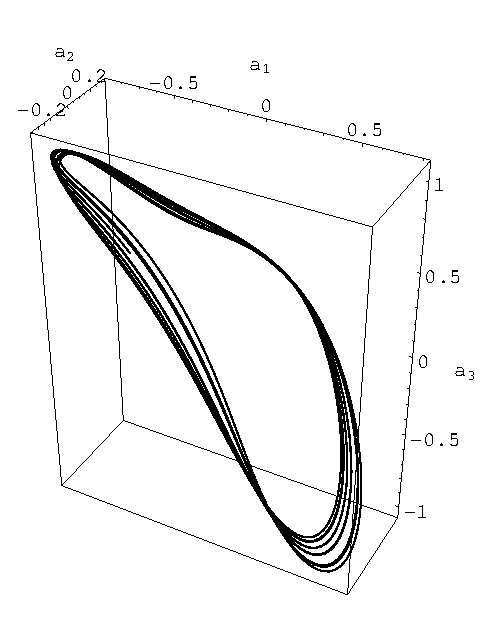
\includegraphics[width=1.8in]{figs/pl1.eps}%
    \hspace{0.2cm}%
    (b)~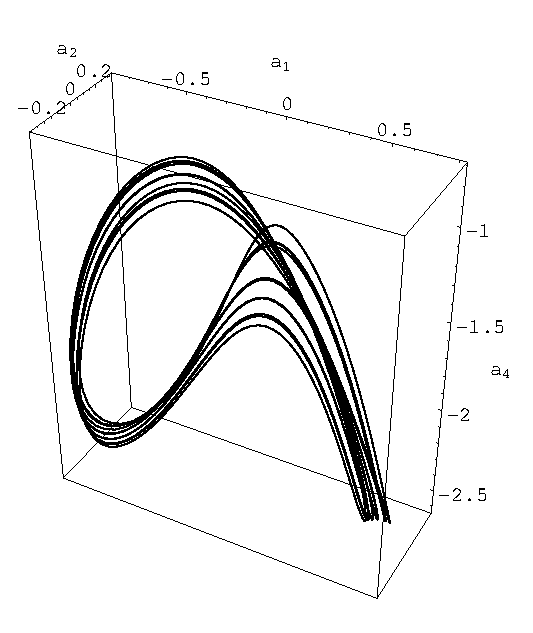
\includegraphics[width=1.8in]{figs/pl2.eps}
    \caption{(a) Projection of a typical trajectory segment onto the {$a_1,a_2,a_3$} subspace.
             (b) Projection of the same trajectory segment onto the {$a_1,a_2,a_4$} subspace. N=16,
                                         $\nu=0.029910$ and $L=2\pi$.
            }
    \label{f:trajectories}
 \end{figure}
%%%%%%%%%%%%%%%%%%%%%%%%%%%%%%%%%%%%%%%%%%%%%%%%%%%%%%%

\subsection{Poincar\'e Section}
\label{sec:poincare}

 To get a feeling for the topology of the attractor we study its Poincar\'e map.
 We choose as the Poincar\'e section the hyperplane $a_1=0$, and follow trajectories
 of the truncated system (\ref{eq:Fcoef Trunc})
 with arbitrary initial conditions on this hyperplane. Each time the trajectory returns
 on the $a_1=0$ hyperplane in the same direction as initially we get a point of the Poincar\'e
 map $(a_2',\ldots,a_N')=P(a_2,\dots,a_N)$. The dynamics is still difficult to
 visualize since the space is $N-1$ dimensional. Yet a plot of the Poincar\'e
 map in a single coordinate as in \reffig{fig:guess} suggests that the attractor for $\nu=0.029910$
 is nearly one dimensional.

 %% \subsection{Implementation Notes}
 %% \label{sec:poincare-numerics}


%%%%%%%%%%%%%%%%%%%%%%%%%%%%%%%%%%%%%%%%%%%%%%%%%%%%%%%%
%\begin{figure}[b!]
%    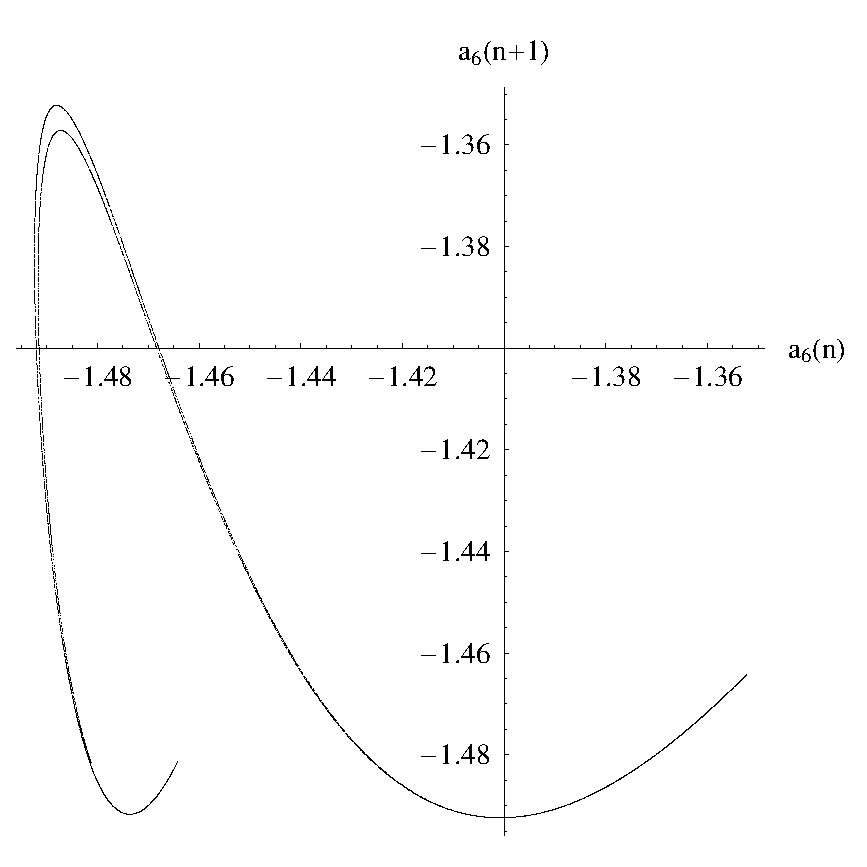
\includegraphics[width=2.5in]{figs/poincare6.eps}%
%    \caption{ $a_1=0$ Poincar\'e section of system (\ref{eq:Fcoef Trunc}) for the $a_6$ coordinate.
%    N=16 Fourier modes truncation and $\nu=0.029910, L=2\pi$. Here 10000 returns to the section are plotted.
%    }
%\label{fig:poincare6}
%\end{figure}
%%%%%%%%%%%%%%%%%%%%%%%%%%%%%%%%%%%%%%%%%%%%%%%%%%%%%%%%%%%%%

\section{Unstable Periodic Orbits}

 \subsection{Formulating an initial guess}

  The first step in finding a periodic orbit of the KS system is
  a good initial guess of a point on such an
  orbit. For the shortest periodic orbits, those that correspond to
  fixed points of the Poincar\'e return map, this is done by considering the Poincar\'e sections of the various
  $a_i$ coefficients. The intersection of the projection of the attractor with
  the line $a_i(n+1)=a_i(n)$ obviously corresponds to a return on the same point
  in the $n$-th coordinate of the Poincar\'e section. If this is the case for all the $a_i$'s then the
  system returns on the same point in the Poincar\'e section, and thus the orbit is
  periodic. We specify an approximate intersection by estimating from Poincar\'e points
  generated by a typical long orbit and use it to initiate Newton's method to find a
  periodic orbit with better precision.

  Yet, as shown in \reffig{fig:guess}(a), the intersection of the bisector and
  the projection of the attractor in a given coordinate may not be unique.
  Apparent intersections are eliminated by checking whether they are close to the
  bisector in other coordinates. If we are lucky (\reffig{fig:guess}(b)), a projection of the
  Poincar\'e section on a particular coordinate is 'good' and singles out the correct intersection
  points.




%
%%%%%%%%%%%%%%%%%%%%%%%%%%%%%%%%%%%%%%%%%%%%%%%%%%%%%%%
 \begin{figure}[t!]
    (a)~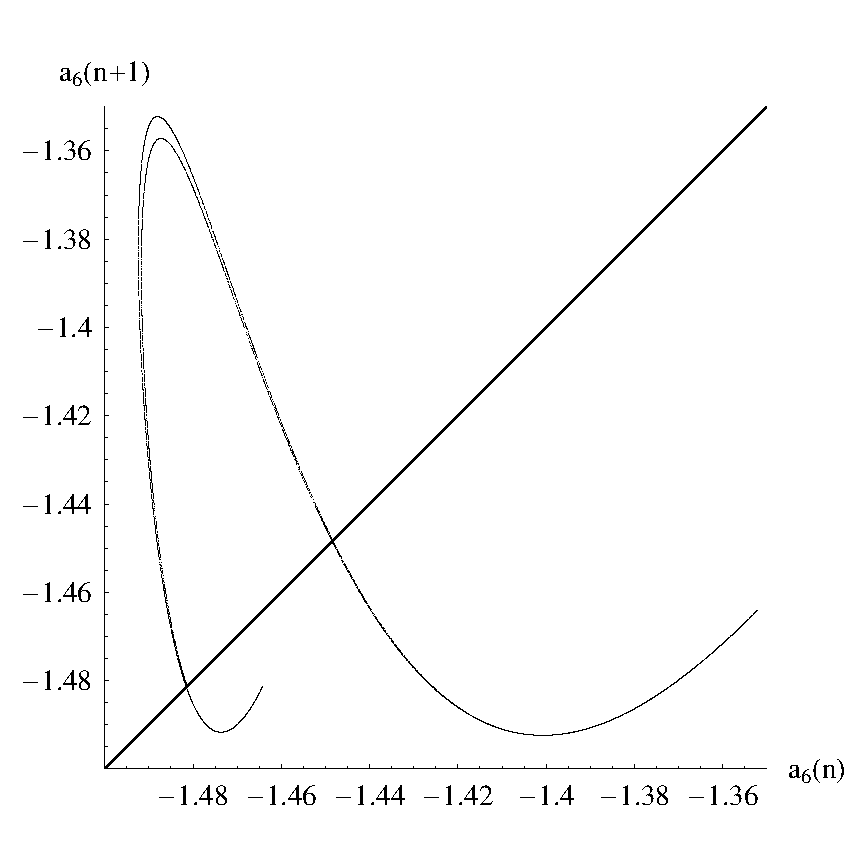
\includegraphics[width=2.2in]{figs/poin6-bi.eps}%
    \hspace{0.2cm}%
    (b)~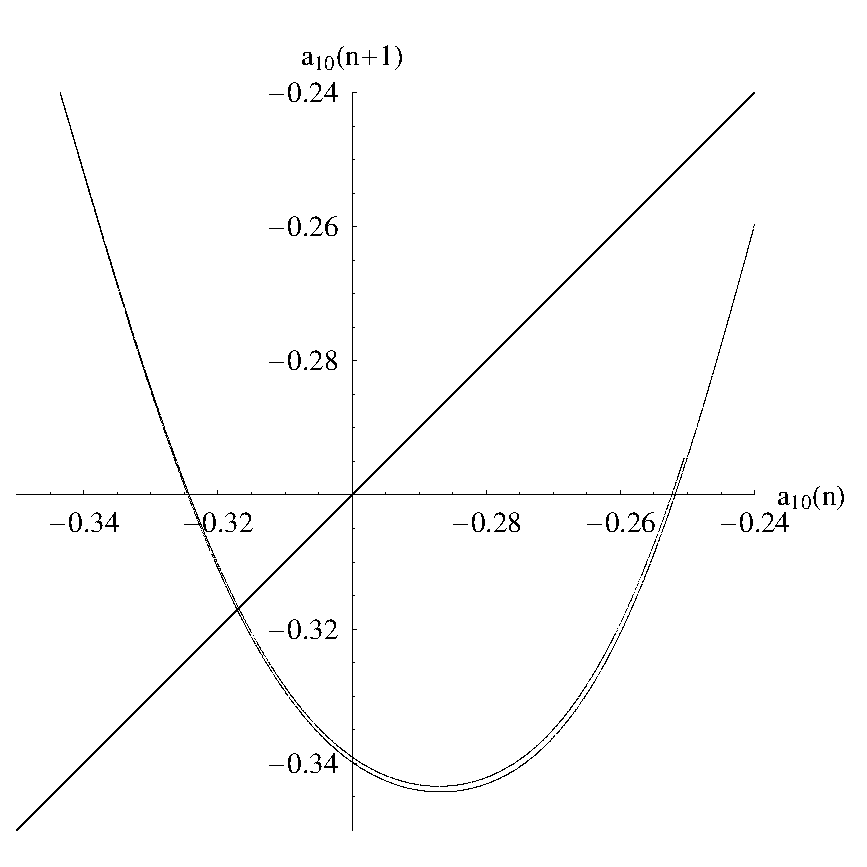
\includegraphics[width=2.2in]{figs/poin10-bi.eps}
    \caption{(a) $a_1=0$ Poincar\'e section of system (\ref{eq:Fcoef Trunc}) for the $a_6$ coordinate.
             (b) $a_1=0$ Poincar\'e section for the $a_{10}$ coordinate.
             N=16 Fourier modes truncation and $\nu=0.029910, L=2\pi$. Here 10000 returns to the section as well as
             the bisector of the axes are plotted.
             }
    \label{fig:guess}
 \end{figure}
%%%%%%%%%%%%%%%%%%%%%%%%%%%%%%%%%%%%%%%%%%%%%%%%%%%%%%%



 \subsection{Implementing Newton's method}

  Newton's method to identify periodic orbits (\cite{DasBuch}, Chapter 15) of an N-dimensional flow $f$
  is based on Newton's method for the solution of a set of nonlinear algebraic equations
  (e.g. \cite{Press:96}, Par. 9.6). We consider a point $x$ lying on a given Poincar\'e section of our system
  and a neighboring point $x'$ not necessarily on the Poincar\'e section. If we integrate
  the flow for a certain time $t$ such that $f^t(x)$ (but not necessarily $f^t(x')$) lies on the Poincar\'e
  section, we can consider a Taylor expansion of $f^t(x')$:
  \beq
    f^t(x') \simeq f^t(x) + \mathbf{J}(x'-x)
    \label{eq:Taylor of Flow}
  \eeq
  where $\mathbf{J}=\mathbf{J}^t(x)$ is the Jacobian matrix defined through (\cite{DasBuch}, Chapter 4):
  \beq
   J^t_{ij}(x_o)=\left.\frac{\partial x_i(t)}{\partial x_j}\right|_{x=x_0}
  \eeq

  The Jacobian matrix is obtained by integrating the equation:
  \beq
   \dot{\mathbf{J}}^t=\mathbf{A J}^t \, ,
   \label{eq:Adef}
  \eeq
  subject to the initial condition:
  \beq
   \mathbf{J}^0=\mathbf{1} \ ,
  \eeq
  starting from $x$ and up to the next intersection with the Poincar\'e section.
  This can be done concurrently with the integration of the equations of the flow,
  using the same integrator. Here $\mathbf{A}$ is the matrix of variations defined as:
  \beq
   A_{kj}=\frac{\partial \dot{a}_k}{\partial a_j}\,.
  \eeq

  We can now require that $x'$ is a fixed point:
  \beq
   f(x')=x'\,
  \eeq
  or with the help of \refeq{eq:Taylor of Flow}:
  \beq
   (1-\mathbf{J})(x'-x)=-(x-f^t(x))\equiv-F(x)\,.
   \label{eq:Newton Algebraic}
  \eeq

  Thus, starting with the initial guess $x$, we can get a better approximation
  $x'$ of a point of a periodic orbit by solving \refeq{eq:Newton Algebraic}.

  A periodic orbit $\mathbf{J}$ always has a unit (marginal) eigenvalue corresponding to
  the direction of the flow, so $\det(1-\mathbf{J})$ evaluated for our initial guess will be numerically very close
  to zero. A determinant equal to zero corresponds to the lack of
  a unique isolated solution, since the periodicity condition holds for the continuous
  family of all points of the periodic orbit.
  The other possibility -- no solution -- is excluded since we assume that
  a periodic orbit exists in the neighborhood of our guess. To establish the uniqueness of a solution further
  constraints on $x'$ are needed, namely the restriction that $x'$ lies on the Poincar\'e section.
  Furthermore, since we want to iterate the procedure improving our estimation of the periodic
  orbit at each step, we would like to
  have $x'$ lying on the Poicar\'e section, so that it would be our next initial guess.
  But if we demand that $x'$ lies on the Poincar\'e section $f^t(x')$ will not in general
  be on that section, since the Jacobian matrix is computed over a time interval
  such that $f^t(x)$ rather than $f^t(x')$ will
  reside on the Poincar\'e section. This would obviously be inconsistent with the periodicity condition $f^t(x')=x'$.
  From a different perspective, demanding that $x'$ and $f(x')$ both lie on the Poincar\'e section
  corresponds to an overspecification of the problem.

  To overcome this difficulty we increase the dimensionality of the problem as follows. We consider
  $f^{t+\delta T}(x)$ with $\delta T$ a small time interval such that $f^{t+\delta T}(x')$ lies on the
  Poincar\'e section. Then we can write:
  \beq
   f^{t+\delta T}(x)=f^t(x)+ v \delta T\,,
   \label{eq:NewtonTimeTaylor}
  \eeq
  where $v=\dot{x}$ is evaluated at $f^t(x)$. % $v \delta T$ being a vector in the direction of the flow

  On the other hand if $f^{t+\delta T}(x')$ lies close enough to $f^{t+\delta T}(x)$ we can write:
  \begin{eqnarray}
   f^{t+\delta T}(x') & \simeq & f^{t+\delta T}(x) +
                                   \mathbf{J}^{t+\delta T}(x)(x'-x)
                                   \label{eq:fapprox:1}  \\
                      & \simeq & f^{t+\delta T}(x) +
                      \mathbf{J}^{t}(x)(x'-x)\,,  \label{eq:fapprox:2}
  \end{eqnarray}
  where in the last step we have used the multiplicative structure of the Jacobian,
  $\mathbf{J}^{t+\delta T}(x)=\mathbf{J}^{\delta T}(f^t(x))\mathbf{J}^{t}(x)$, noticed that
  $\mathbf{J}^{\delta T}(f^t(x))=e^{\mathbf{A}\delta T}=\mathbf{1}+\mathbf{A}\delta T+\ldots$ and dropped second order terms in the small quantities.

  Thus, because of \refeq{eq:NewtonTimeTaylor}:
  \beq
    f^{t+\delta T}(x') \simeq f^{t}(x) + v \delta T + \mathbf{J}^{t}(x)(x'-x)\,.
    \label{eq:Ext Newton Algebraic}
  \eeq

  The last equation, along
  with the periodicity requirement for $x'$, $f^{t+\delta T}(x')=x'$ reads:
  \beq
   (1-\mathbf{J}^{t}(x))(x'-x)-v \delta T = -(x-f^t(x))\equiv -F(x)\,.
  \eeq
    We now can demand that $x'$ be on the Poincar\'e section,
    since we then can adjust the undetermined time $\delta T$ so as to have $f^{t+\delta T}(x')$ on the Poincar\'e
    section. If the latter is an hyperplane we have the condition:
    \beq
     a \cdot (x-x')=0
     \label{eq:Poincare}
    \eeq
    where a is a vector normal to that hyperplane (and $x$ is already assumed on the hyperplane).
    Equations \refeq{eq:Ext Newton Algebraic} and \refeq{eq:Poincare} can be compactly represented
    in a single matrix equation:
    \beq
    \left( \begin{array}{cc}
       1-\mathbf{J}^{t}(x) & v \\
       a & 0 \\
     \end{array}
     \right)
     \left(\begin{array}{c}
       x'-x \\
       \delta T \\
     \end{array}\right)
     =
     \left(\begin{array}{c}
       -F(x) \\
       0     \\
     \end{array}\right)\,,
     \label{eq:NewtonScheme}
    \eeq
   where we have absorbed a minus sign in $\delta T$. Solving this equation for the corrections $\delta x = x'-x$
   and $\delta T$ yields a better estimation to (a point of) the periodic orbit and its period $t-\delta T$.

  Returning to the KS equation
  we get from \refeq{eq:Fcoef Trunc} and \refeq{eq:Adef}:
  \beq
   A_{kj}=\left(\frac{2\pi}{L}\right)^2\left(k^2- \left(2\pi/L\right)\nu k^4\right)\delta_{kj}
            -\frac{4\pi}{L} k\left(a_{k-j}-a_{k+j} \right)\,.
  \eeq

  Using the initial guess for the cycle $\overline{1}$ (the symbolic dynamics are to be explained in
  a subsequent section) from \reffig{fig:guess} Newton's
  method now yields the  actual cycle, with the return to the initial point accurate up to
  $10^{-13}$. The solution of the linear system is carried out by QR-decomposition, using the algorithms
  given in ref. \cite{Press:96}, Chapter B9.

  The four largest eigenvalues of the Jacobian matrix for the cycle $\overline{1}$ are shown in
  \reftab{tab:Jeigen}. The difference of the marginal eigenvalue $\Lambda_2$ from unity is indicative
  (at least in a loose sense) of the accuracy of the numerical calculation.

  \begin{table}[h!]
\begin{tabbing}
    Cycle \=  -2.014326 aaa \=  $1.1 \cdot 10^{-10}$ aaaa \=  $6.579608 \cdot 10^{-3}$ aaaa \= $-3.653655 \cdot 10^{-4}$ aaaa \= \kill
    Cycle \> Period         \> $\Lambda_1$  \>  $1-\Lambda_2$           \> $\Lambda_3$                  \> $\Lambda_4$  \\
    $\overline{1}$     \> 0.870729       \> -2.014327    \>  $1.4 \cdot 10^{-13}$    \> $6.579608 \cdot 10^{-3}$     \> $-3.653655 \cdot 10^{-4}$ \\
    $\overline{10}$    \> 1.751810       \> -3.801854    \>  $-1.2\cdot 10^{-12}$    \> $-3.892045\cdot 10^{-5}$     \> $ 2.576622\cdot 10^{-7}$

\end{tabbing}
\caption{The period and the four largest stability eigenvalues for cycles $\overline{1}$ and $\overline{10}$.
            N=16 and $\nu=0.029910,\ L=2\pi$ .}
   \label{tab:Jeigen}
  \end{table}

\subsection{Multipoint Shooting Method}

 Periodic orbits with $n$ Poincar\'e section returns are found with
 the Multipoint Shooting Method (\cite{DasBuch}, Chapter 15). For
 $n=2$ initial guesses are formulated by examing the map of second return on the Poincar\'e section.
 The results for the cycle $\overline{10}$ are shown in \reftab{tab:Jeigen}.



\subsection{Unstable Manifold of the $ \overline{1}$   cycle \label{sec:UnstableManifold}}

 The unstable manifold of a fixed point $x_o$ of a flow consists of all the
 points that approach $x_o$, under the action of the flow, but with the
 direction of time inversed, $t\rightarrow -\infty$. For an infinitesimal neighborhood of the
 fixed point, this property pertains to the unstable eigendirections of the
 flow. Thus, as any point of the unstable manifold is carried by the
 time-reversed flow towards the fixed point, it will eventually land
 on it through one of its unstable eigendirections. Reversing the
 process we can place a large number of initial conditions on an
 infinitesimal segment of an unstable eigendirection and get a finite
 segment of the unstable manifold by letting the flow transport those
 initial conditions.

 In the case of the  $ \overline{1}$ cycle of the KS system we observe
 that there is only one unstable eigendirection, given by the
 eigendirection that corresponds to $\Lambda_1$. Thus, we can get a
 picture of its unstable manifold by placing a collection of
 initial conditions $x_i$ on the Poincar\'e section and along
 this direction according to:
 \beq
  x_i=x_o+\lambda_i \hat{j}_1\, ,
  \label{eq:unstable initialization}
 \eeq
 where $\hat{j}_1$ the projection of the unstable eigenvector on the
 Poincar\'e section $a_1=0$ and $\lambda_i$ a
 parameter varied in small steps, so that we do not end up far away
 from $x_o$.

 The $a_6$ coordinate projection of the
 unstable manifold is shown in \reffig{fig:Manifold}.
 We observe that the unstable manifold is indistinguishable from the
 strange attractor of \reffig{fig:guess}(a). It exhibits a fractal structure, yet it is very thin -- nearly
 one-dimensional. Furthermore the projection shown is clearly
 a non single-valued function, while in some other projections
 the manifold appears to be self-intersecting. The dynamics of the system cannot easily be
 understood in terms of such curves. The origin of the problem is that
 the Poincar\'e map of the unstable manifold is a curve embedded in a
 higher dimensional space  ($ 2\times(N-1)$--dimensional) and what we see in plots like
 \reffig{fig:Manifold} is a projection of this curve in two
 dimensions. We discuss a way out of this difficulty in the
 next section.

 %%%%%%%%%%%%%%%%%%%%%%%%%%%%%%%%%%%%%%%%%%%%%%%%%%%%%%%%
 \begin{figure}[b!]
     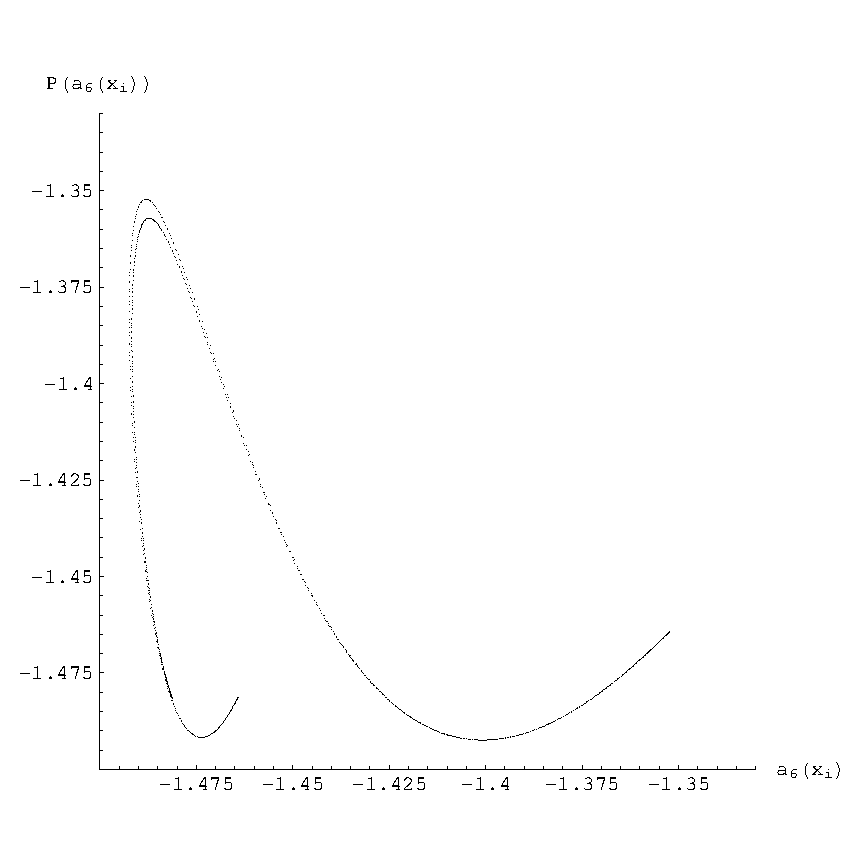
\includegraphics[width=3.5in]{figs/manifold.eps}
     \caption{ $a_1=0$ Poincar\'e section of the unstable manifold of $ \overline{1}$   cycle  for the $a_6$ coordinate.
     N=16 Fourier modes truncation, $\nu=0.029910, L=2\pi$. The
     plot was generated by using 1400 initial conditions on the
     unstable eigendirection of the cycle and iterating each of them
     12 times. To improve the resolution near the ``folding points'',
     $\lambda_i$ in \refeq{eq:unstable initialization} was varied in
     steps of the form $\Delta\lambda_i=\pm 3\cdot 10^{-6}\, \exp(-10^{-3}\,i)$.
     }
 \label{fig:Manifold}
 \end{figure}
 %%%%%%%%%%%%%%%%%%%%%%%%%%%%%%%%%%%%%%%%%%%%%%%%%%%%%%%%%%%%%



 \subsubsection{Unstable Manifold Parametrization}

  In \cite{Christiansen:97} it was shown that parametrizing the unstable manifold with
  the help of a length $s$ measured on the full-dimensional space
  results on a (nearly) single-valued Poincar\'e map   $s(n) \rightarrow
  s(n+1)$. Such a parametrization of the
  unstable manifold will be presented here, carried out in a slightly
  different way.

  First, we observe that the fractal structure of the unstable
  manifold results from its folding at two points of the curve. The
  reason for this is that the strange attractor is confined in a
  finite region of the phase space, while the unstable manifold is, by
  its definition, infinite.
  % Discuss the connection to the deterministic character of the flow
  This is undesirable, since we would like to be able to map a
  point of a given trajectory to exactly one point on the manifold to
  which we will assign a unique length $s$. Using a curve that densely
  folds on itself means that two closely situated points of a
  trajectory can be mapped on two distant points on the unstable
  manifold (in the sense of distance along the curve).

  To overcome this difficulty we need to identify the two nearest ``folding points'' and only
  use the part of the manifold between them. Obviously on those
  points the curvature of the curve on the Poincar\'e section of
  \reffig{fig:Manifold} becomes very large compared to the curvature
  on the other points. The curvature at a point can be approximated by
  using its two neighboring points and determining the radius of the
  circle that passes through them (using the expressions found e.g. in
  \cite{circle}). The curvature will then be the
  inverse of this radius. This way we can get a plot of the curvature at
  each point of the curve, with sharp peaks identifying the folding
  points.

  Next we compute the Euclidean distance between the
  adjacent points $(\Delta s_i)^2=\sum_{k=1}^N \left(a_k(x_i)-a_k(x_{i-1})\right)^2$ and,
  setting $s=0$ at $x_o$ we compute
  the distance $s(x_i)=s_i=\sum_{k=1}^i \Delta s_k $ for each point on the manifold, so that points
  at the left (right) of $x_o$ have negative (possitive) $s$.

  Having parametrized the unstable manifold this way, we can follow a
  sample trajectory and assign to each point of intersection with the
  Poincar\'e section the value of $s$ of the closest point on the
  unstable manifold. By closest point we mean the one with the minimum distance
  from a given trajectory point. This allows us to construct the return map
  $s(n)\rightarrow s(n+1)$ for the trajectory, which is shown in
  \reffig{fig:sPoincare}. We observe that -- miraculously-- the map
  resembles a parabola! There is fractal structure to the map but the
  thickness is very small and we can treat the curve as
  one-dimensional and single valued. This feature of the return map
  is very helpful in constructing the symbolic dynamics, cf. ref. \cite{Christiansen:97}.

  %%%%%%%%%%%%%%%%%%%%%%%%%%%%%%%%%%%%%%%%%%%%%%%%%%%%%%%%
  \begin{figure}[h!]
      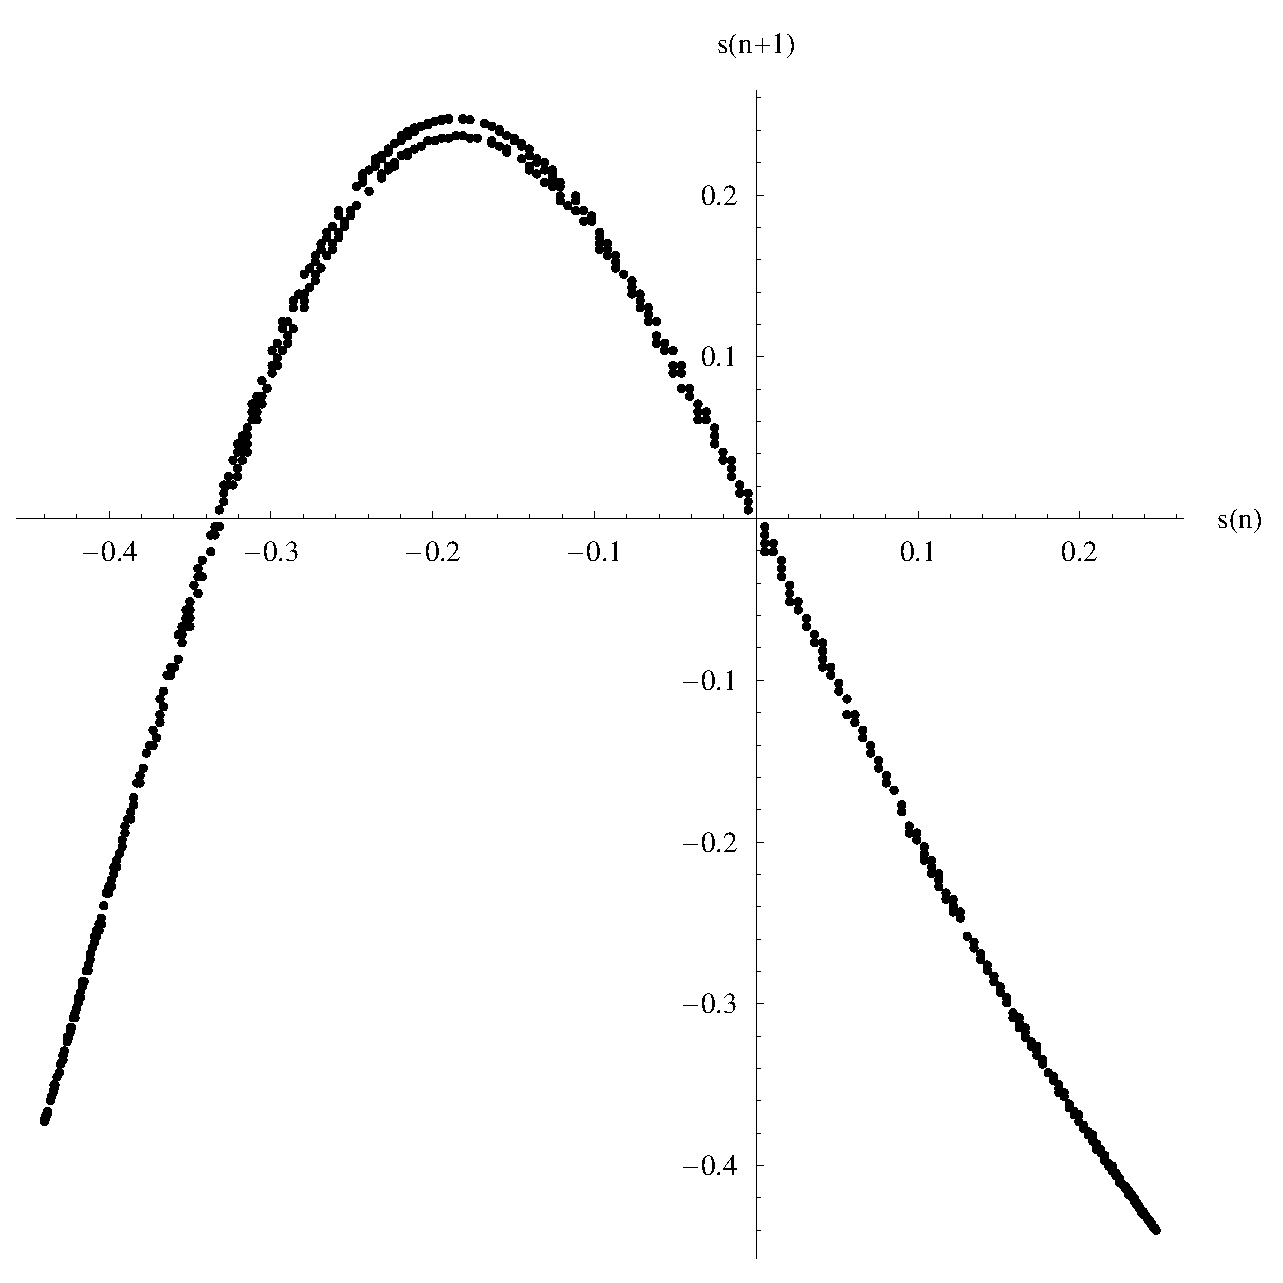
\includegraphics[width=4in]{figs/sPoincarePlot.eps}
      \caption{ $a_1=0$ Poincar\'e section of a typical trajectory in
        the $s$ parametrization. N=16 Fourier modes truncation,
        $\nu=0.029910, L=2\pi$,1000 points of the sample trajectory.
        To construct the map, a segment of the
        unstable manifold discretized by 240 points was used.
      }
  \label{fig:sPoincare}
  \end{figure}
  %%%%%%%%%%%%%%%%%%%%%%%%%%%%%%%%%%%%%%%%%%%%%%%%%%%%%%%%%%%%%



 \subsection{Linear analysis of the flow}


  We begin by considering the coordinate system defined by the
  eigendirections $\hat{\mathbf{e}}_j$ of $\mathbf{J}_o \equiv\mathbf{J}^{T_o}(x_o)$,
  where $x_o$ the central fixed point, on the intersection of the unstable manifold
  and diagonal in \reffig{fig:guess}(a). This is a good
  coordinate system only
  if the $\hat{\mathbf{e}}_j$ are linearly independent (or,
  equivalently, $\mathbf{J}_o$ is diagonalizable by a similarity
  transformation).   For the KS system we easily confirm numerically the linear independence of the
  $\hat{\mathbf{e}}_j$.  %% could we see it on the structure of J ?
  In general the $\hat{\mathbf{e}}_j$'s
  do not form an orthogonal basis; in case at hand, $\mathbf{J}_o$ is not
  symmetric, cf. \refappe{appe:DiagJ}.

  We then consider the hypersurface $\mathcal{P}$ which can be written
  in the $\hat{\mathbf{a}}_i$ basis as:
  \beq
   x=x_o+\sum_{i=1}^{N-1}\, q_i\, \hat{\mathbf{e}}_i \, ,
  \eeq
  with the understanding that the $N$'th eigendirection is the
  marginal one. Thus, the $q_i$'s are just the coordinates of point on
  $\mathcal{P}$ in the
  $\hat{e}_i$ basis. We then conclude that a small neighborhood of $x_o$ on $\mathcal{P}$ will be
  transported by the flow after time $t_o=m\,T_o$, where $m$ is an integer
  and $T_o$ the period of the prime cycle at $x_o$,
  to:
  \beq
       f^{t_o}(x) = f^{t_o}\left(x_o+\sum_{i=1}^{N-1}\, q_i\, \hat{\mathbf{e}}_i\right) \,
  \eeq
  Taylor expanding for small $q_i's$:
  \beq
       f^{t_o}(x) = f^{t_o}(x_o) + \mathbf{J}^{t_o}(x_o)
       \sum_{i=1}^{N-1}\, q_i\, \hat{\mathbf{e}}_i + \mathcal{O}\left(q_i^2\right)    \, ,
     \label{eq:lin flow P}
  \eeq
  The motivation for this choice of Poincar\'e section was to avoid
  an extra term arising from the fact that the first return time is
  different for each trajectory for an arbitrary Poincar\'e section. Yet
  this difficulty can be easily overcome by other means,
  \cf ref. \cite{DasBuch}.

  Because of the multiplicative structure of the Jacobian matrix
  we have:
  \beq
   \mathbf{J}^{t_o}(x_o)=(\mathbf{J}^{T_o}(x_o))^m \equiv
                \mathbf{J}_o^m \,,
  \eeq
  and \refeq{eq:lin flow P} reads:
  \begin{eqnarray}
       f^{t_o}(x)          & \simeq & f(x_o) + \mathbf{J}_o^m
           \sum_{i=1}^{N-1}\, q_i\, \hat{\mathbf{e}}_i    \, ,
         \\                  & = & x_o + \sum_{i=1}^{N-1}\,\Lambda_i^m\, q_i\,
                    \hat{\mathbf{e}}_i  \, , \label{eq:f stays on P}
  \end{eqnarray}
  where we have used $f^{t_o}(x_o)=x_o$ and the eigenvalue-eigenvector
  equation for $\mathbf{J_p}$:
  \beq
   \mathbf{J}_o\, \hat{\mathbf{e}}_i = \Lambda_i \hat{\mathbf{e}}_i\, ,
  \eeq

  The seperation after time $t$ of
  two points on $\mathcal{P}$ initially in the neighborhood of $x_o$
  is seen to be:
  \begin{eqnarray}
    \delta f & = &  f^{t_o}(x_k)-f^{t_o}(x_j) \\
             & = &  \sum_{i=1}^{N-1}\,\Lambda_i^m\, q^{(k)}_i\,
               \hat{\mathbf{e}}_i -
               \sum_{i=1}^{N-1}\,\Lambda_i^m\, q^{(j)}_i\,
               \hat{\mathbf{e}}_i \\
             & = & \sum_{i=1}^{N-1}\,\Lambda_i^m\, \delta q_i \,
               \hat{\mathbf{e}}_i \, ,
  \end{eqnarray}
  where the superscripts $(j)$ refer to the different initial points.
  Thus if we express $\delta f$ in the $\hat{\mathbf{e}}_i$ basis
  $\delta f = \sum_{i=1}^{N-1}\, \delta \tilde{f}_i \,
               \hat{\mathbf{e}}_i =  \sum_{i=1}^{N-1}\, \left( \left(\delta f-x_o\right)\,\cdot \hat{\mathbf{e}}_i \right)
               \hat{\mathbf{e}}_i $ we get:
  \beq
    \sum_{i=1}^{N-1}\, \left(\delta \tilde{f}_i \,  - \Lambda_i^m\, \delta q_i \,
               \right) \hat{\mathbf{e}}_i =0\, .
  \eeq
  Since the $\hat{\mathbf{e}}_i$ are assumed linearly independent  we immediately get:
  \beq
    \delta \tilde{f}_i \, = \Lambda_i^m\, \delta q_i \, .
    \label{eq:delta f}
  \eeq
  Or, using $x_o$ (which is the origin for the $\hat{\mathbf{e}}_j$
  coordinate system) as one of the points:
  \beq
   \tilde{f}_i(x)=\Lambda_i^m q_i
   \label{eq:delta f sp}
  \eeq
  Thus, we can track the orbit of a point $x$ in the vicinity of $x_o$
  just by multiplying each of its initial coordinates (in the
  $\hat{\mathbf{e}}_j$ basis) by  the corresponding eigenvalue of $\mathbf{J}_o$ raised in the
  $m$'th power for the $m$'th return to $\mathcal{P}$. The change of basis
  from $\hat{\mathbf{e}}_i$ to $\hat{\mathbf{a}}_i$ can then be
  easilly performed. Of course, this analysis is valid only for points
  in the infinitesimal neighborhood of $x_o$, where the nonlinear
  terms can be safely neglected.


\section{The metric tensor on the unstable manifold}

 The Euclidean metric used to measure the distance along the unstable manifold
 is only a possible one. A better one should be natural to the
 flow, and a good candidate is:
 \beq
  \mathbf{g}=\mathbf{J}^T(x)\mathbf{J}(x)
 \eeq
 where $\mathbf{J}^T$ is the transpose of $\mathbf{J}$, and no time
 index has been assigned to $\mathbf{J}$ since it is not clear for
 what time interval should $\mathbf{J}$ be computed for non periodic
 orbits.


\section{Conclussion}

 During the project a part of the results of \cite{Christiansen:97}
 was reproduced, while the unstable manifold parametrization was
 carried out in an alternative way. On the other hand, periodic orbit
 theory was not actually used to perform cycle expansions since that
 requires the determination of more cycles. The parametrization of the
 unstable manifold, though, makes the search for cycles easier, since
 it essentially reduces the symbolic dynamics to that of the unimodal map.
 Yet, the determination of longer cycles was postponed by the search for a better metric for the
 system, which I think is an interesting open question.

 %%%%%%%%%%%%%%%%%%%%%%%%%%%%%%%%%%%%%%%%%%%%%%%%%%%%%%%%%%%%





%%%%%%%%%%%%%%%%%%%%%%%%%%%%%%%%%%%%%%%%%%%%%%%%%%%%%%%%%%%%%

%%%%%%%% Bibliography

 \bibliographystyle{unsrt}
 \bibliography{nameless.bib}
 \nocite{*}

\end{document}
